\begin{exercise}
      {ID-79763e9291ca3e4cfb33b1f0e1ee05d24c620d41}
      {Gateway-Arch}
  \ifproblem\problem\par
    % <PROBLEM>
    Der Gateway-Arch (1959--1965 gebaut) in St.\,Louis, Missouri, ist laut
    Angaben eines Reiseführers ein parabelförmiger Bogen aus rostfreiem
    Stahl. Er ist 630 Fuß (\emph{ft}) hoch und an seiner breitesten Stelle
    ebenso breit. Er soll als \glqq{}Tor zum Westen\grqq{} an den nach 1800
    einsetzenden Siedlerstrom nach Westen in den USA erinnern.
    \begin{enumerate}[a)]
      \item Wie breit ist der Bogen in 300\,\emph{ft} Höhe (in \emph{ft})?
      \item 1\,\emph{ft} entspricht \simeter{0.3048}. Bestimme eine
            Funktionsgleichung mit der man die Höhe des Gateway-Arch in Metern
            beschreiben kann.
      \item Bei einer Flugshow soll ein Flugzeug mit einer Flügelspannweite
            von \simeter{18} unter dem Bogen hindurch fliegen. Welche maximale
            Flughöhe muss der Pilot einhalten, wenn in vertikaler und horizontaler
            Richtung ein Sicherheitsabstand zum Bogen von \simeter{10} eingehalten
            werden muss?
    \end{enumerate}
    % </PROBLEM>
  \fi
  %\ifoutline\outline\par
    % <OUTLINE>
    % </OUTLINE>
  %\fi
  \ifoutcome\outcome
    % <OUTCOME>
    \begin{enumerate}[a)]
      \item Wenn man den Ursprung des Koordinatensystems
            in die Mitte des Bauwerks auf Bodenhöhe
            legt, besitzt die Funktion, die die Parabel
            beschreibt, ihren Scheitelpunkt bei
            $\left(0\;\middle|\;630\right)$ und zwei
            Nullstellen bei $\left(-315\;\middle|\;0\right)$
            und $\left(315\;\middle|\;0\right)$.
            Mit diesen Informationen lässt sich die
            Funktionsgleichung bestimmen:
            \begin{equation*}
              \begin{split}
                f(x)&=a\cdot(x-0)^2+630=ax^2+630
                \\
                0&=a\cdot315^2+630
                \\[1ex]
                \Rightarrow\quad
                a&=-\frac{630}{315^2}=-\frac{2}{315}
              \end{split}
            \end{equation*}
            Um die Breite in \num{300}\,\textit{ft}
            Höhe bestimmen zu können, muss man
            zunächst die $x$-Werte finden, bei
            denen sich der $y$-Wert \num{300}
            ergibt.
            \begin{alignat*}{3}
              \relax&\quad
              &
              300&=-\frac{2}{315}\cdot x^2+630
              &
              \quad&|-300
              \\[1ex]
              \Leftrightarrow&\quad
              &
              0&=-\frac{2}{315}\cdot x^2+330
              &
              \quad&|:\left(-\frac{2}{315}\right)
              \\[1ex]
              \Leftrightarrow&\quad
              &
              0&=x^2-\num{51975}
              &
              \quad&\relax
              \\[1ex]
              \relax&\quad
              &
              x_1&=-\sqrt{\num{51975}}\approx-\num{227.98}
              &
              \quad&\relax
              \\
              \relax&\quad
              &
              x_2&=\sqrt{\num{51975}}\approx\num{227.98}
              &
              \quad&\relax
            \end{alignat*}
            Der Gateway-Arch ist also in \num{300}\,\textit{ft}
            Höhe etwa \num{455.96}\,\textit{ft} breit.
      \item Um in der Einheit Meter rechnen zu könmem,
            muss die Funktion $f$ sowohl in $x$-
            als auch in $y$-Richtung gestaucht
            werden. Alle bisher berechneten Höhen
            hatten die Einheit Fuß. Folgende
            Transformation liefert Höhen in der
            Einheit Meter:
            \begin{equation*}
              g(x)=\num{0.3048}\cdot f(x)
            \end{equation*}
            Alle bisher eingesetzten horizontalen
            Entfernungen hatten ebenfalls die Einheit Fuß.
            Folgende Transformation ermöglicht es zusätzlich
            auch die $x$-Werte in der Einheit Meter einsetzen
            zu können:
            \begin{equation*}
              g(x)=\num{0.3048}\cdot f(x:\num{0.3048})
            \end{equation*}
            Man erhält also insgesamt folgende Funktion:
            \begin{equation*}
              \begin{split}
                g(x)&=\num{0.3048}\cdot
                \left(
                  -\frac{2}{315}\cdot
                  \left(
                    \frac{x}{\num{0.3048}}
                  \right)^2
                  +630
                \right)
                \\[1ex]
                &=-\frac{2}{315\cdot\num{0.3048}}\cdot x^2
                  +\num{630}\cdot\num{0.3048}
                \\[1ex]
                &=-\frac{167}{\num{8017}}\cdot x^2
                 +\frac{\num{24003}}{\num{125}}
                \approx-\num{0.021}x^2+\num{192.024}
                %rats(-2 / (315 * 0.3048))
                %rats(630 * 0.3048)
              \end{split}
            \end{equation*}
      \item Der Sicherheitsbereich um das Flugzeug
            herum hat die Form eines Rechtecks:
            \begin{center}
              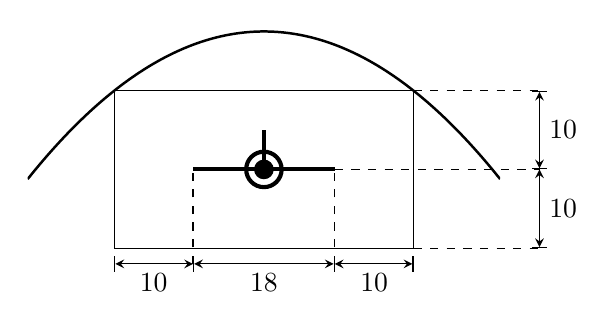
\begin{tikzpicture}
                \begin{scope}[line width=1.5pt]
                  \draw (-9mm, 0) -- (9mm, 0);
                  \draw (0, 0) -- (0, 5mm);
                  \fill (0, 0) circle[radius=1.25mm];
                  \draw (0, 0) circle[radius=2.25mm];
                \end{scope}
                % Sicherheitsbereich
                \draw (-19mm, -10mm) rectangle (19mm, 10mm);
                % Hilfslinien
                \draw[style=dashed] (-9mm, -12mm) -- (-9mm, 0mm);
                \draw[style=dashed] ( 9mm, -12mm) -- ( 9mm, 0mm);
                % Hilfslinien horizontal
                \draw[style=dashed] (19mm,  10mm) -- (35mm,  10mm);
                \draw[style=dashed] ( 9mm,   0mm) -- (35mm,   0mm);
                \draw[style=dashed] (19mm, -10mm) -- (35mm, -10mm);
                % Beschriftung unten
                \begin{scope}[yshift=-12mm, >=stealth]
                  \draw[|<->]  (-19mm, 0) -- node[below]{\SI{10}{\metre}} (-9mm, 0);
                  \draw[|<->|] ( -9mm, 0) -- node[below]{\SI{18}{\metre}} ( 9mm, 0);
                  \draw[<->|]  (  9mm, 0) -- node[below]{\SI{10}{\metre}} (19mm, 0);
                \end{scope}
                % Beschriftung rechts
                \begin{scope}[xshift=35mm, >=stealth]
                  \draw[|<->|] (0, 0) -- node[right]{\SI{10}{\metre}} (0,  10mm);
                  \draw[<->|]  (0, 0) -- node[right]{\SI{10}{\metre}} (0, -10mm);
                \end{scope}
                % Gateway-Arch
                \begin{scope}[scale=0.1, line width=0.9pt]
                  \clip (-30.000, -2.000) rectangle (30.000, 18.000);
                  \draw plot[smooth] coordinates
                  {
                    (-30.000,  -1.228) (-29.000,   0.001) (-28.000,   1.189)
                    (-27.000,   2.334) (-26.000,   3.438) (-25.000,   4.501)
                    (-24.000,   5.521) (-23.000,   6.500) (-22.000,   7.438)
                    (-21.000,   8.334) (-20.000,   9.188) (-19.000,  10.000)
                    (-18.000,  10.771) (-17.000,  11.500) (-16.000,  12.187)
                    (-15.000,  12.833) (-14.000,  13.437) (-13.000,  14.000)
                    (-12.000,  14.520) (-11.000,  14.999) (-10.000,  15.437)
                    ( -9.000,  15.833) ( -8.000,  16.187) ( -7.000,  16.499)
                    ( -6.000,  16.770) ( -5.000,  16.999) ( -4.000,  17.187)
                    ( -3.000,  17.332) ( -2.000,  17.437) ( -1.000,  17.499)
                    (  0.000,  17.520) (  1.000,  17.499) (  2.000,  17.437)
                    (  3.000,  17.332) (  4.000,  17.187) (  5.000,  16.999)
                    (  6.000,  16.770) (  7.000,  16.499) (  8.000,  16.187)
                    (  9.000,  15.833) ( 10.000,  15.437) ( 11.000,  14.999)
                    ( 12.000,  14.520) ( 13.000,  14.000) ( 14.000,  13.437)
                    ( 15.000,  12.833) ( 16.000,  12.187) ( 17.000,  11.500)
                    ( 18.000,  10.771) ( 19.000,  10.000) ( 20.000,   9.188)
                    ( 21.000,   8.334) ( 22.000,   7.438) ( 23.000,   6.500)
                    ( 24.000,   5.521) ( 25.000,   4.501) ( 26.000,   3.438)
                    ( 27.000,   2.334) ( 28.000,   1.189) ( 29.000,   0.001)
                    ( 30.000,  -1.228)
                  };
                \end{scope}
              \end{tikzpicture}
            \end{center}
            Die maximale Flughöhe erhält man, indem
            man von der Höhe, in der der Gateway-Arch
            eine Breite von \SI{38}{\metre} besitzt,
            den vertikalen Sicherheitsabstand
            von \SI{10}{\metre} abzieht:
            \begin{equation*}
              g(-19)=g(19)\approx\num{184.44}
              %g = [-0.021 0 192.024];
              %polyval(g, -19)
              %polyval(g,  19)
              \quad\Rightarrow\quad
              h_{\text{max}}\approx\num{174.44}
            \end{equation*}
            Wenn es der Pilot schafft, genau die Mitte
            des Gateway-Arch zu treffen, darf er nicht
            höher als \SI{174.44}{\metre} fliegen.
    \end{enumerate}
    % </OUTCOME>
  \fi
\end{exercise}
